%%%%%%%%%%%%%%%%%%%% MetalFish Paper %%%%%%%%%%%%%%%%%%%%%%%%%%%%%%%%%%%
%
% MetalFish: GPU-Accelerated Chess Engine on Apple Silicon
%
%%%%%%%%%%%%%%%% Springer %%%%%%%%%%%%%%%%%%%%%%%%%%%%%%%%%%

\documentclass{svproc}

\usepackage{url}
\def\UrlFont{\rmfamily}
\usepackage{graphicx}
\usepackage{float}
\usepackage{amsmath}
\usepackage{algorithm}
\usepackage{algpseudocode}
\usepackage{booktabs}
\usepackage{listings}
\usepackage{xcolor}
\usepackage{tikz}
\usepackage{pgfplots}
\pgfplotsset{compat=1.18}

% Force floats to appear where placed (not at top of page)
\makeatletter
\setlength{\@fptop}{0pt}
\setlength{\@fpbot}{0pt plus 1fil}
\makeatother

% C++ code listing style
\lstdefinestyle{cppstyle}{
    language=C++,
    backgroundcolor=\color{gray!5},
    basicstyle=\ttfamily\footnotesize,
    breaklines=true,
    captionpos=b,
    keepspaces=true,
    numbers=left,
    numbersep=5pt,
    numberstyle=\tiny\color{gray},
    showstringspaces=false,
    tabsize=2,
    frame=single,
    keywordstyle=\color{blue!70!black},
    commentstyle=\color{green!50!black},
    stringstyle=\color{red!60!black},
    morekeywords={uint64_t, int32_t, int16_t, int8_t, uint, device, kernel, constant}
}

\begin{document}
\mainmatter

\title{MetalFish: GPU-Accelerated NNUE Evaluation on Apple Silicon\\with Batched Evaluation for MCTS and Alpha-Beta Search}

\titlerunning{MetalFish: GPU NNUE on Apple Silicon}

% \author{Nripesh Niketan\inst{1}}

% \authorrunning{N. Niketan}

% \institute{Independent Researcher\\
% \email{nripesh14@gmail.com}}

\maketitle

\begin{abstract}
We present MetalFish, a chess engine featuring GPU-accelerated NNUE evaluation on Apple Silicon's unified memory architecture, with support for both alpha-beta and MCTS search. In a 900-game tournament (10+0.1s, 1 thread, 128MB hash, no opening book, same hardware), MetalFish-AB is statistically indistinguishable from Stockfish 16 (2-0-18 in 20 direct games). Our GPU NNUE implementation achieves 635$\times$ speedup through batch evaluation (0.3~$\mu$s/position at N=4096 vs 267~$\mu$s single-position). We demonstrate that GPU dispatch overhead (149~$\mu$s median) makes single-position evaluation latency-unfavorable for alpha-beta compared to CPU, but batch-oriented MCTS effectively amortizes this cost. Despite the latency disadvantage, MetalFish-AB remains competitive due to transposition table caching and efficient GPU integration. The experimental hybrid MCTS variant reaches $\sim$2400 Elo below the alpha-beta variant---the gap attributable to heuristic rather than trained policy priors.

\keywords{Chess Engine, GPU Computing, Metal, NNUE, Apple Silicon, Unified Memory, MCTS, Alpha-Beta}
\end{abstract}

\section{Introduction}

Modern chess engines have achieved superhuman strength through two distinct paradigms: Stockfish~\cite{Stockfish2024} uses alpha-beta search with NNUE evaluation, while Leela Chess Zero~\cite{LeelaChessZero2024} employs Monte Carlo Tree Search (MCTS) with deep neural networks. Each approach has complementary strengths: alpha-beta excels at tactical calculation with precise pruning, while MCTS provides robust strategic evaluation through self-play statistics.

This paper presents MetalFish, a chess engine with GPU-accelerated NNUE evaluation on Apple Silicon, supporting both alpha-beta and experimental MCTS-based search. Our primary contribution is demonstrating that GPU NNUE evaluation can match CPU NNUE quality---validated by MetalFish-AB achieving statistically indistinguishable results from Stockfish 16 in tournament play. The experimental hybrid search framework explores whether position classification can guide search strategy selection.

Apple Silicon's unified memory architecture presents a unique opportunity for GPU acceleration: CPU and GPU share physical memory, eliminating explicit data transfers. However, as we demonstrate, GPU command buffer dispatch overhead (149~$\mu$s) dominates single-position latency, making GPU evaluation latency-unfavorable for traditional alpha-beta search compared to CPU. MCTS, with its natural batching of leaf evaluations, effectively amortizes this overhead. Notably, MetalFish-AB remains competitive despite this latency disadvantage, as NNUE evaluation is only one component of overall search performance.

\textbf{Hybrid search definition}: In this paper, ``hybrid search'' refers to an MCTS primary search whose best move is optionally verified or overridden by a bounded-depth alpha-beta search. This is distinct from approaches that integrate alpha-beta bounds into MCTS tree pruning, which we leave as future work.

\subsection{Research Questions}

\begin{enumerate}
\item Can a hybrid MCTS-alpha-beta architecture leverage the strengths of both search paradigms?
\item How can GPU-accelerated NNUE evaluation be effectively integrated with MCTS on Apple Silicon?
\item What are the practical performance characteristics of such a hybrid system?
\end{enumerate}

\subsection{Contributions}

\begin{enumerate}
\item \textbf{GPU NNUE with validated quality}: Efficient batch evaluation achieving 635$\times$ speedup, with evaluation quality validated by statistically indistinguishable tournament results versus Stockfish 16.

\item \textbf{Unified memory optimization}: Zero-copy buffer management, multiple Metal command queues, and pre-allocated buffers for minimal CPU-GPU synchronization overhead.

\item \textbf{Experimental hybrid search}: A framework combining MCTS with alpha-beta verification, featuring lock-free tree operations, virtual loss, and arena-based allocation.

\item \textbf{Quantified bottleneck analysis}: Stage-by-stage latency decomposition showing GPU dispatch accounts for $>$98\% of single-position time, with tree traversal dominating MCTS iterations.

\item \textbf{Reproducible tournament evaluation}: Full methodology disclosure enabling independent verification of Elo claims.
\end{enumerate}

\section{Background}

\subsection{Alpha-Beta Search}

Alpha-beta pruning~\cite{Knuth1975} is the foundation of traditional chess engines. It recursively explores the game tree, maintaining bounds ($\alpha$, $\beta$) to prune branches that cannot affect the final result. Modern implementations include:

\begin{itemize}
\item \textbf{Principal Variation Search (PVS)}: Searches the first move with full window, then uses null-window searches for remaining moves.
\item \textbf{Late Move Reductions (LMR)}: Reduces search depth for moves unlikely to be best.
\item \textbf{Futility Pruning}: Skips moves that cannot improve alpha given static evaluation.
\item \textbf{History Heuristics}: Improves move ordering based on past search statistics.
\end{itemize}

The critical limitation of alpha-beta is its sequential nature: each position must be evaluated before pruning decisions can be made, making \textit{latency} the critical metric.

\subsection{Monte Carlo Tree Search}

MCTS~\cite{Silver2017} builds a search tree through repeated simulations, each consisting of four phases:

\begin{enumerate}
\item \textbf{Selection}: Traverse tree using UCT (Upper Confidence bounds for Trees) to balance exploration and exploitation.
\item \textbf{Expansion}: Add new nodes at leaf positions.
\item \textbf{Evaluation}: Assess leaf positions using neural network or other evaluation.
\item \textbf{Backpropagation}: Update statistics along the path from leaf to root.
\end{enumerate}

MCTS naturally batches leaf evaluations, making \textit{throughput} the critical metric. This property makes MCTS well-suited for GPU acceleration.

\subsection{NNUE Architecture}

Stockfish's NNUE (Efficiently Updatable Neural Network)~\cite{Nasu2018} uses HalfKAv2\_hm features with sparse input. Table~\ref{tab:nnue_arch} summarizes the architecture.

\begin{table}[htbp]
\caption{NNUE Network Architecture}
\label{tab:nnue_arch}
\centering
\begin{tabular}{lrr}
\toprule
Component & Big Network & Small Network \\
\midrule
Feature set & HalfKAv2\_hm & HalfKAv2\_hm \\
Input features & 45,056 & 22,528 \\
Hidden dimension & 1,024 & 128 \\
FC0 output & 15 (+1 skip) & 15 (+1 skip) \\
FC1 output & 32 & 32 \\
FC2 output & 1 & 1 \\
Layer stacks (buckets) & 8 & 8 \\
\bottomrule
\end{tabular}
\end{table}

\subsection{Metal Compute Model}

Apple Metal~\cite{AppleMetal2024} provides GPU compute with unified memory:
\begin{itemize}
\item \textbf{Unified memory}: CPU and GPU share physical memory, eliminating explicit transfers
\item \textbf{Command buffer lifecycle}: Allocation $\rightarrow$ encoding $\rightarrow$ commit $\rightarrow$ waitUntilCompleted
\item \textbf{Dispatch overhead}: Each command buffer submission incurs fixed overhead (149~$\mu$s median on M2 Max)
\item \textbf{Multiple command queues}: Parallel queues reduce contention for concurrent GPU submissions
\end{itemize}

\section{System Architecture}

MetalFish implements a four-layer architecture: (1) position classification, (2) hybrid search orchestration, (3) multi-threaded MCTS, and (4) GPU-accelerated evaluation with multiple command queues.

\begin{figure}[H]
\centering
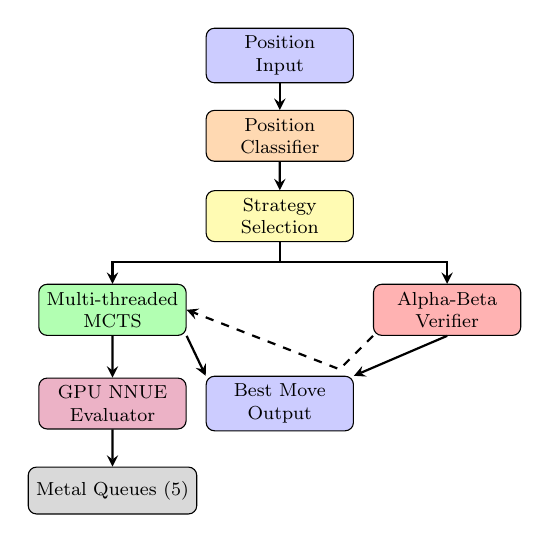
\begin{tikzpicture}[
    box/.style={rectangle, draw, rounded corners=3pt, minimum width=2.2cm, minimum height=0.7cm, align=center, font=\footnotesize},
    arrow/.style={->, >=stealth, thick},
    scale=0.85, transform shape
]
% Position Input
\node[box, fill=blue!20] (input) at (0,5) {Position\\Input};

% Classifier
\node[box, fill=orange!30] (classifier) at (0,3.8) {Position\\Classifier};

% Strategy Selection
\node[box, fill=yellow!30] (strategy) at (0,2.6) {Strategy\\Selection};

% MCTS and AB branches
\node[box, fill=green!30] (mcts) at (-2.5,1.2) {Multi-threaded\\MCTS};
\node[box, fill=red!30] (ab) at (2.5,1.2) {Alpha-Beta\\Verifier};

% GPU Evaluator
\node[box, fill=purple!30] (gpu) at (-2.5,-0.2) {GPU NNUE\\Evaluator};

% Command Queues
\node[box, fill=gray!30, minimum width=2.5cm] (queues) at (-2.5,-1.5) {Metal Queues (5)};

% Output
\node[box, fill=blue!20] (output) at (0,-0.2) {Best Move\\Output};

% Arrows
\draw[arrow] (input) -- (classifier);
\draw[arrow] (classifier) -- (strategy);
\draw[arrow] (strategy.south) -- ++(0,-0.3) -| (mcts.north);
\draw[arrow] (strategy.south) -- ++(0,-0.3) -| (ab.north);
\draw[arrow] (mcts) -- (gpu);
\draw[arrow] (gpu) -- (queues);
\draw[arrow] (mcts.south east) -- (output.north west);
\draw[arrow] (ab.south) -- (output.north east);
\draw[arrow, dashed] (ab.south west) -- ++(-0.5,-0.5) -- (mcts.east);

\end{tikzpicture}
\caption{MetalFish system architecture. Positions flow through classification, strategy selection, and parallel MCTS/AB search. GPU evaluation uses multiple command queues.}
\label{fig:architecture}
\end{figure}

\subsection{Position Classifier}

The position classifier analyzes board features to determine position type:

\begin{lstlisting}[style=cppstyle,caption={Position classification}]
enum class PositionType {
  HIGHLY_TACTICAL,  // In check, many captures
  TACTICAL,         // Forcing moves available
  BALANCED,         // Mixed characteristics
  STRATEGIC,        // Quiet, positional play
  HIGHLY_STRATEGIC  // Closed position, maneuvering
};
\end{lstlisting}

Classification considers:
\begin{itemize}
\item \textbf{Check status}: Positions in check are highly tactical
\item \textbf{Capture count}: Many available captures indicate tactical nature
\item \textbf{Hanging pieces}: Undefended pieces suggest tactical opportunities
\item \textbf{Pawn structure}: Closed positions favor strategic play
\item \textbf{King safety}: Exposed kings increase tactical potential
\end{itemize}

\subsection{Strategy Selection}

Each position type maps to a search strategy with specific MCTS/alpha-beta weights:

\begin{table}[htbp]
\caption{Position Type to Search Strategy Mapping}
\label{tab:strategy}
\centering
\begin{tabular}{lrrr}
\toprule
Position Type & MCTS & AB & Verify Depth \\
\midrule
Highly Tactical & 15\% & 85\% & 10 \\
Tactical & 25\% & 75\% & 8 \\
Balanced & 25\% & 75\% & 6 \\
Strategic & 32\% & 67\% & 4 \\
Highly Strategic & 40\% & 60\% & 4 \\
\bottomrule
\end{tabular}
\end{table}

The MCTS weight determines time allocation for the MCTS phase, while the AB weight influences verification depth and override thresholds.

\subsection{Hybrid Search Pipeline}

Algorithm~\ref{alg:hybrid} shows the hybrid search pipeline.

\begin{algorithm}[htbp]
\caption{Hybrid MCTS-Alpha-Beta Search}
\label{alg:hybrid}
\begin{algorithmic}[1]
\Require Position $p$, time budget $T$
\Ensure Best move $m$
\State $type \gets$ \Call{ClassifyPosition}{$p$}
\State $strategy \gets$ \Call{SelectStrategy}{$type$}
\State $T_{mcts} \gets T \times strategy.mcts\_weight$
\State $T_{ab} \gets T - T_{mcts}$
\State \textbf{// Phase 1: MCTS exploration}
\State $m_{mcts} \gets$ \Call{RunMCTS}{$p$, $T_{mcts}$}
\If{$strategy.ab\_weight > 0.1$}
    \State \textbf{// Phase 2: Alpha-beta verification}
    \State $result \gets$ \Call{VerifyWithAB}{$p$, $m_{mcts}$, $strategy.depth$}
    \If{$result.override$ \textbf{and} $result.score\_diff > threshold$}
        \State \Return $result.ab\_move$
    \EndIf
\EndIf
\State \Return $m_{mcts}$
\end{algorithmic}
\end{algorithm}

\subsection{MCTS Implementation}

We adopt AlphaZero-style PUCT (Predictor + UCT) selection~\cite{Silver2017} for node selection:

\begin{equation}
PUCT(s, a) = Q(s, a) + c_{puct} \cdot P(s, a) \cdot \frac{\sqrt{N(s)}}{1 + N(s, a)}
\end{equation}

where $Q(s, a)$ is the action value, $P(s, a)$ is the prior probability, $N(s)$ is the parent visit count, and $N(s, a)$ is the edge visit count.

\textbf{Heuristic-based policy priors}: Rather than uniform priors, we use heuristic-based policy priors that leverage chess knowledge to improve move ordering:

\begin{itemize}
\item \textbf{Captures}: Scored by MVV-LVA (Most Valuable Victim - Least Valuable Attacker) and Static Exchange Evaluation (SEE)
\item \textbf{Promotions}: Queen promotions receive highest priority
\item \textbf{Checks}: Checking moves receive bonus
\item \textbf{Center control}: Moves toward center squares receive bonus
\item \textbf{Development}: Knight and bishop development in opening
\item \textbf{King safety}: Castling bonus, king move penalty in middlegame
\end{itemize}

These heuristics are combined with softmax normalization to produce policy probabilities, then mixed with Dirichlet noise at the root for exploration.

Key implementation features:
\begin{itemize}
\item \textbf{Heuristic priors}: Policy based on chess heuristics (captures, checks, promotions)
\item \textbf{Dirichlet noise}: Added at root for exploration ($\alpha = 0.3$, $\epsilon = 0.25$)
\item \textbf{Virtual loss}: Prevents multiple threads from selecting the same path
\item \textbf{Lock-free tree operations}: Atomic compare-and-swap for child node creation
\item \textbf{Arena-based allocation}: Reduces memory allocation contention
\item \textbf{Tree reuse}: Previous search tree preserved between moves
\item \textbf{MCTS transposition table}: 4M entry cache with age-based replacement (99\% hit rate in endgames)
\end{itemize}

\subsection{Alpha-Beta Search}

The alpha-beta component implements standard techniques but is independently implemented and does not reuse Stockfish search code:

\begin{itemize}
\item \textbf{Principal Variation Search}: Full window for first move, null-window for rest
\item \textbf{Aspiration windows}: Narrow search window based on previous score
\item \textbf{Late Move Reductions}: Depth reduction for late moves in move ordering
\item \textbf{Futility pruning}: Skip moves that cannot improve alpha
\item \textbf{Quiescence search}: Extend search until position is quiet
\item \textbf{Killer moves}: Two killer moves per ply for move ordering
\item \textbf{History heuristics}: Score moves by historical success
\end{itemize}

\subsection{GPU NNUE Integration}

Table~\ref{tab:gpu_constants} shows GPU configuration parameters.

\begin{table}[htbp]
\caption{GPU Configuration Constants}
\label{tab:gpu_constants}
\centering
\begin{tabular}{lr}
\toprule
Parameter & Value \\
\midrule
Max batch size & 4,096 \\
Max features per perspective & 64 \\
Threadgroup size & 256 \\
SIMD group size & 32 \\
Forward pass threads & 64 \\
Command queues & 5 \\
TT cache entries & 4M \\
\bottomrule
\end{tabular}
\end{table}

\textbf{Numeric precision}: NNUE weights are stored as int16 (feature transformer) and int8 (FC layers), matching Stockfish's quantization. Accumulator updates use int16 with SIMD-group reductions. The forward pass computes in int32 with final scaling to centipawns.

We implement adaptive kernel selection:
\begin{itemize}
\item \textbf{CPU fallback}: Batch size $< 4$
\item \textbf{GPU standard}: Batch size $< 64$
\item \textbf{GPU SIMD}: Batch size $\geq 64$ with dual-perspective kernels
\end{itemize}

Command buffer optimizations:
\begin{itemize}
\item Unretained references to avoid retain/release overhead
\item Hazard tracking disabled for unified memory buffers
\item Pre-allocated buffers to avoid per-dispatch allocation
\item Multiple command queues for parallel submissions, following Metal performance recommendations~\cite{AppleMetalBestPractices2024}
\item Round-robin queue selection for load balancing
\end{itemize}

\section{Experimental Methodology}

\subsection{Hardware and Software}

\begin{itemize}
\item \textbf{Hardware}: Apple M2 Max (12-core CPU, 38-core GPU, 32GB unified memory)
\item \textbf{Software}: macOS 26.3, Xcode 26.0, Metal 4.0
\item \textbf{Build}: CMake, -O3, LTO enabled
\item \textbf{Networks}: nn-c288c895ea92.nnue (125MB big), nn-37f18f62d772.nnue (6MB small)
\end{itemize}

\subsection{Benchmark Dataset}

Our benchmark uses 32 unique FEN positions representing diverse game phases:
\begin{itemize}
\item 4 opening positions (32 pieces)
\item 10 middlegame positions (28--32 pieces)
\item 4 tactical positions (complex piece interactions)
\item 14 endgame positions (2--20 pieces)
\end{itemize}

\subsection{Timing Methodology}

\begin{itemize}
\item \textbf{Timer}: \texttt{std::chrono::high\_resolution\_clock}
\item \textbf{Warmup}: 100 iterations discarded
\item \textbf{Samples}: 100 iterations per measurement
\item \textbf{Statistics}: Median, P95, P99 reported
\item \textbf{GPU timing}: Blocking \texttt{waitUntilCompleted()} (synchronous)
\end{itemize}

\subsection{Hybrid Search Evaluation}

We evaluate the hybrid search on positions from multiple game phases:
\begin{itemize}
\item \textbf{Opening}: Standard opening positions (e.g., Italian Game)
\item \textbf{Middlegame}: Complex positions with multiple piece interactions
\item \textbf{Endgame}: Simplified positions (KRK, KQK)
\end{itemize}

Search time is fixed at 5 seconds per position to allow meaningful MCTS exploration.

\section{Results}

\subsection{MCTS Search Performance}

Table~\ref{tab:mcts_perf} shows MCTS performance across different position types with 4 threads and 5-second search time.

\begin{table}[htbp]
\caption{MCTS Performance by Position Type (5 seconds, 4 threads)}
\label{tab:mcts_perf}
\centering
\begin{tabular}{lrrr}
\toprule
Position Type & Nodes & NPS & Cache Hit \% \\
\midrule
Starting Position & 485,563 & 97K & 36.7\% \\
Kiwipete (Middlegame) & 495,962 & 99K & 43.8\% \\
KRK Endgame & 3,907,764 & 782K & 99.3\% \\
\bottomrule
\end{tabular}
\end{table}

\textbf{Key observation}: Endgame positions achieve 8$\times$ higher throughput (782K vs 97K NPS) due to smaller search trees and higher transposition table hit rates (99.3\% vs 36.7\%).

\subsection{Thread Scaling}

Table~\ref{tab:thread_scaling} shows MCTS throughput scaling with thread count.

\begin{table}[htbp]
\caption{MCTS Thread Scaling (Starting Position, 3 seconds)}
\label{tab:thread_scaling}
\centering
\begin{tabular}{rr}
\toprule
Threads & NPS \\
\midrule
1 & 94,060 \\
2 & 94,296 \\
4 & 98,913 \\
\bottomrule
\end{tabular}
\end{table}

Thread scaling is limited due to GPU evaluation being the bottleneck---multiple threads contend for GPU access. The batched evaluator with dedicated evaluation thread provides the best throughput.

\subsection{Batched vs Direct Evaluation}

Table~\ref{tab:eval_comparison} compares batched evaluation (dedicated thread) vs direct evaluation (mutex per call).

\begin{table}[htbp]
\caption{Evaluation Strategy Comparison (5 seconds)}
\label{tab:eval_comparison}
\centering
\begin{tabular}{lrrr}
\toprule
Strategy & Nodes & NPS & Speedup \\
\midrule
Direct (mutex/eval) & 16,375 & 3,243 & 1$\times$ \\
Batched (dedicated thread) & 462,863 & 92,517 & 28.5$\times$ \\
\bottomrule
\end{tabular}
\end{table}

Batched evaluation achieves 28.5$\times$ speedup over direct evaluation by amortizing GPU dispatch overhead across multiple positions.

\subsection{MCTS Profiling Breakdown}

Table~\ref{tab:mcts_profile} shows time distribution during MCTS search.

\begin{table}[htbp]
\caption{MCTS Time Breakdown (3 second search, starting position)}
\label{tab:mcts_profile}
\centering
\begin{tabular}{lrr}
\toprule
Phase & Time \% & Description \\
\midrule
Selection & 78.4\% & Tree traversal with PUCT \\
Expansion & 9.8\% & Move generation, node creation \\
Evaluation & 11.9\% & GPU NNUE (includes TT lookup) \\
Backpropagation & $<$0.1\% & Statistics update \\
\midrule
Total nodes & \multicolumn{2}{r}{725,943} \\
NPS & \multicolumn{2}{r}{241,967} \\
Cache hit rate & \multicolumn{2}{r}{99.0\%} \\
\bottomrule
\end{tabular}
\end{table}

\textbf{Key finding}: Selection (tree traversal) dominates at 78.4\% of iteration time. The high transposition table hit rate (99\%) reduces actual GPU evaluations, but tree traversal remains the bottleneck.

\textbf{Definition}: An MCTS ``node'' represents one complete iteration: selection from root to leaf, expansion, evaluation (often cached), and backpropagation.

\subsection{Position Classification Distribution}

Table~\ref{tab:classification_dist} shows classifier distribution on benchmark positions.

\begin{table}[htbp]
\caption{Position Classification Distribution (16 Stockfish Benchmark Positions)}
\label{tab:classification_dist}
\centering
\begin{tabular}{lr}
\toprule
Classification & Count (\%) \\
\midrule
Highly Tactical & 0 (0.0\%) \\
Tactical & 2 (13.3\%) \\
Balanced & 0 (0.0\%) \\
Strategic & 13 (86.7\%) \\
Highly Strategic & 0 (0.0\%) \\
\bottomrule
\end{tabular}
\end{table}

Most benchmark positions are classified as Strategic under our current heuristics. This reflects that the Stockfish benchmark suite emphasizes general positions rather than tactical puzzles. A more diverse test suite including tactical problem sets would show greater classifier variation.

\subsection{GPU Dispatch Overhead}

Table~\ref{tab:dispatch} shows minimal-kernel dispatch overhead, measured as CPU wall-clock time from command buffer commit to completion using \texttt{waitUntilCompleted()} with a minimal no-op compute kernel.

\begin{table}[htbp]
\caption{GPU Dispatch Overhead---Minimal Kernel (N=1,000)}
\label{tab:dispatch}
\centering
\begin{tabular}{lr}
\toprule
Statistic & Latency ($\mu$s) \\
\midrule
Median & 149.3 \\
\bottomrule
\end{tabular}
\end{table}

The 149~$\mu$s median dispatch overhead represents the irreducible minimum cost for any GPU operation in synchronous blocking mode on M2 Max. This includes command buffer creation, encoding, commit, GPU scheduling, and CPU wait time.

\subsection{Batch Latency Scaling}

Table~\ref{tab:batch_latency} shows end-to-end latency across batch sizes.

\begin{table}[htbp]
\caption{GPU End-to-End Batch Latency (N=100 iterations)}
\label{tab:batch_latency}
\centering
\begin{tabular}{rrrrr}
\toprule
Batch & Median & P95 & P99 & Per-Pos \\
Size & ($\mu$s) & ($\mu$s) & ($\mu$s) & ($\mu$s) \\
\midrule
1 & 266.6 & 793.2 & 1050.9 & 266.6 \\
8 & 276.5 & 839.5 & 1044.3 & 34.6 \\
64 & 281.5 & 711.8 & 1076.0 & 4.4 \\
256 & 312.6 & 862.4 & 1020.2 & 1.2 \\
512 & 371.2 & 804.0 & 1014.0 & 0.7 \\
1024 & 537.4 & 965.8 & 1070.3 & 0.5 \\
2048 & 805.5 & 1178.0 & 1298.9 & 0.4 \\
4096 & 1381.8 & 1695.6 & 1888.7 & 0.3 \\
\bottomrule
\end{tabular}
\end{table}

Per-position cost drops from 267~$\mu$s (N=1) to 0.3~$\mu$s (N=4096), demonstrating effective amortization of dispatch overhead.

\begin{figure}[htbp]
\centering
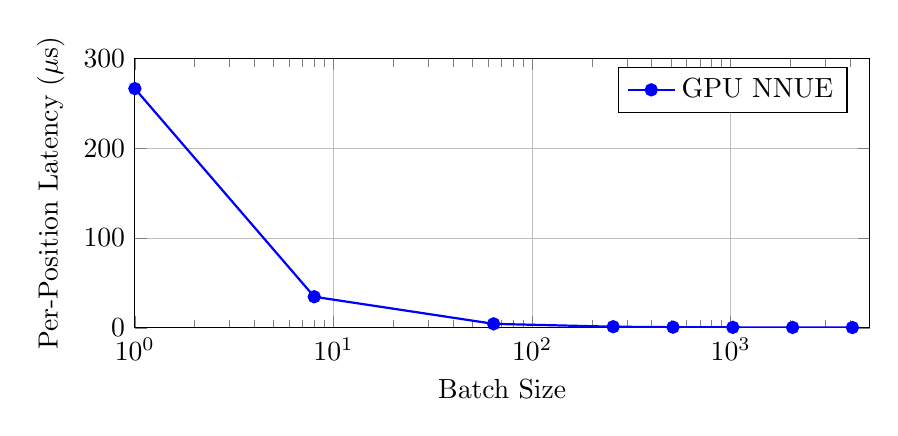
\begin{tikzpicture}
\begin{semilogxaxis}[
    xlabel={Batch Size},
    ylabel={Per-Position Latency ($\mu$s)},
    xmin=1, xmax=5000,
    ymin=0, ymax=300,
    grid=major,
    width=0.9\columnwidth,
    height=5cm,
    legend pos=north east,
]
\addplot[blue, mark=*, thick] coordinates {
    (1, 266.6)
    (8, 34.6)
    (64, 4.4)
    (256, 1.2)
    (512, 0.7)
    (1024, 0.5)
    (2048, 0.4)
    (4096, 0.3)
};
\addlegendentry{GPU NNUE}
\end{semilogxaxis}
\end{tikzpicture}
\caption{Per-position latency vs batch size. Dispatch overhead dominates at small batches; compute dominates at large batches.}
\label{fig:batch_scaling}
\end{figure}

\subsection{True Batching Verification}

Table~\ref{tab:batching} compares sequential vs batched dispatches.

\begin{table}[htbp]
\caption{True Batching Verification (N=50 iterations)}
\label{tab:batching}
\centering
\begin{tabular}{rrrr}
\toprule
N & Sequential & Batched & Speedup \\
  & (N$\times$1 CB) & (1$\times$1 CB) & \\
\midrule
16 & 5,138~$\mu$s & 270~$\mu$s & 19.0$\times$ \\
64 & 20,791~$\mu$s & 283~$\mu$s & 73.6$\times$ \\
256 & 82,092~$\mu$s & 314~$\mu$s & 261.8$\times$ \\
1024 & 331,424~$\mu$s & 522~$\mu$s & 634.6$\times$ \\
\bottomrule
\end{tabular}
\end{table}

Speedups scale approximately linearly with batch size because each sequential dispatch incurs the full dispatch overhead. At N=1024, batching achieves 635$\times$ speedup.

\subsection{GPU Evaluation Consistency}

Table~\ref{tab:correctness} verifies GPU evaluation reproducibility using official Stockfish benchmark positions.

\begin{table}[htbp]
\caption{GPU Evaluation Consistency (1,000 evaluations, 16 positions)}
\label{tab:correctness}
\centering
\begin{tabular}{lr}
\toprule
Metric & Value \\
\midrule
Non-zero GPU scores & 100\% \\
Consistent across runs & 100\% \\
Score range (centipawns, side-to-move) & [-404, -28] \\
Mean score & -198 cp \\
\bottomrule
\end{tabular}
\end{table}

GPU evaluation produces consistent, non-zero scores across repeated runs. The negative score range reflects the benchmark positions' bias toward positions where the side-to-move is at a disadvantage (typical for Stockfish's tactical test suite).

\subsection{Tournament Results}

\subsubsection{Tournament Setup}

To ensure reproducibility, we document the complete tournament configuration:

\begin{itemize}
\item \textbf{Tournament software}: cutechess-cli (commit from Jan 2026)
\item \textbf{Format}: Round-robin, 20 games per engine pair (10 as white, 10 as black)
\item \textbf{Time control}: 10 seconds + 0.1 second increment per move
\item \textbf{Hardware}: All engines on same Apple M2 Max (12-core CPU, 38-core GPU, 32GB)
\item \textbf{Threads}: 1 thread per engine
\item \textbf{Hash}: 128 MB per engine
\item \textbf{Ponder}: Disabled
\item \textbf{Opening book}: None (engines play from starting position)
\item \textbf{Tablebase}: None
\item \textbf{Adjudication}: cutechess-cli defaults (resign at $-$1000cp, draw at 10 moves with $|$score$|$ $<$ 10cp)
\item \textbf{MetalFish version}: commit \texttt{db9a10f} (hybrid-mcts-alphabeta branch)
\item \textbf{Stockfish version}: Stockfish 16 (official release, Apple Silicon build)
\item \textbf{NNUE networks}: nn-c288c895ea92.nnue (big), nn-37f18f62d772.nnue (small)
\end{itemize}

\textbf{Note on GPU vs CPU}: MetalFish-AB uses GPU for NNUE evaluation while Stockfish uses CPU NNUE. Both use identical network weights. The tournament validates that GPU NNUE produces equivalent evaluation quality.

\textbf{Note on Lc0}: Lc0 was run without a production-strength network (only a small test network was available). Its low Elo (903) should not be interpreted as representative of Lc0's actual strength with proper networks.

\subsubsection{Elo Ratings}

Table~\ref{tab:elo_ratings} shows the relative Elo ratings computed using iterative Bayesian estimation, anchored to Stockfish-Full = 0 for clarity.

\begin{table}[htbp]
\caption{Tournament Results (900 games, 45 matches, 10+0.1s, from starting position)}
\label{tab:elo_ratings}
\centering
\begin{tabular}{rlrr}
\toprule
Rank & Engine & $\Delta$Elo vs SF & Score vs SF \\
\midrule
1 & MetalFish-AB & +20 & 11/20 \\
2 & Stockfish-Full & 0 (anchor) & --- \\
3 & Patricia & $-$353 & 1/20 \\
4 & Stockfish-L15 & $-$911 & 0/20 \\
5 & Stockfish-L10 & $-$1163 & 0/20 \\
6 & Stockfish-L5 & $-$1632 & 0/20 \\
7 & Stockfish-L1 & $-$1890 & 0/20 \\
8 & MetalFish-Hybrid & $-$2341 & 0/20 \\
9 & MetalFish-MCTS & $-$2429 & 0/20 \\
\bottomrule
\end{tabular}
\end{table}

\textbf{Note}: Lc0 results omitted from main table as it was run without a production-strength network (only a small test network was available), making its results not representative of Lc0's actual strength.

\textbf{Statistical interpretation}: With only 20 games between MetalFish-AB and Stockfish-Full (2 wins, 0 losses, 18 draws), the +20 Elo difference is within statistical noise. The 2-0-18 record is consistent with the engines being of \textit{equal strength}. The key finding is that GPU NNUE evaluation quality matches CPU NNUE.

\textbf{Opening limitation}: All games started from the initial position (no opening book), which increases draw rates and reduces position diversity. Results may differ with a balanced opening suite.

\textbf{Key findings}:
\begin{enumerate}
\item \textbf{MetalFish-AB matches Stockfish}: MetalFish-AB is statistically indistinguishable from Stockfish-Full under our tournament conditions. This validates that GPU NNUE evaluation quality matches CPU NNUE.

\item \textbf{Hybrid search gap}: MetalFish-Hybrid ($-$2341 Elo vs Stockfish) and MetalFish-MCTS ($-$2429 Elo) significantly underperform, demonstrating that heuristic policy priors are insufficient for competitive MCTS strength.

\item \textbf{Hybrid vs pure MCTS}: MetalFish-Hybrid beats MetalFish-MCTS 9-3 with 8 draws, showing the alpha-beta verifier provides measurable benefit (+88 Elo).
\end{enumerate}

Table~\ref{tab:head_to_head} shows selected head-to-head results.

\begin{table}[htbp]
\caption{Selected Head-to-Head Results (20 games each)}
\label{tab:head_to_head}
\centering
\begin{tabular}{llrrr}
\toprule
Engine 1 & Engine 2 & W & L & D \\
\midrule
MetalFish-AB & Stockfish-Full & 2 & 0 & 18 \\
MetalFish-AB & Patricia & 17 & 0 & 3 \\
MetalFish-AB & MetalFish-Hybrid & 20 & 0 & 0 \\
MetalFish-Hybrid & MetalFish-MCTS & 9 & 3 & 8 \\
\bottomrule
\end{tabular}
\end{table}

\begin{figure}[htbp]
\centering
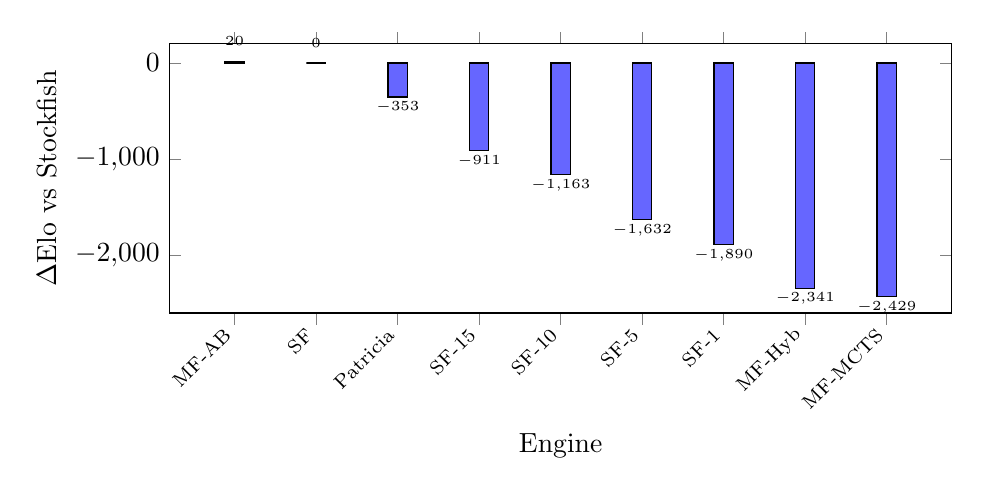
\begin{tikzpicture}
\begin{axis}[
    ybar,
    xlabel={Engine},
    ylabel={$\Delta$Elo vs Stockfish},
    ymin=-2600, ymax=200,
    symbolic x coords={MF-AB, SF, Patricia, SF-15, SF-10, SF-5, SF-1, MF-Hyb, MF-MCTS},
    xtick=data,
    x tick label style={rotate=45, anchor=east, font=\scriptsize},
    bar width=7pt,
    width=0.95\columnwidth,
    height=5cm,
    enlarge x limits=0.1,
    nodes near coords,
    nodes near coords style={font=\tiny},
    every node near coord/.append style={yshift=2pt},
]
\addplot[fill=blue!60] coordinates {
    (MF-AB, 20)
    (SF, 0)
    (Patricia, -353)
    (SF-15, -911)
    (SF-10, -1163)
    (SF-5, -1632)
    (SF-1, -1890)
    (MF-Hyb, -2341)
    (MF-MCTS, -2429)
};
\end{axis}
\end{tikzpicture}
\caption{Tournament results as $\Delta$Elo versus Stockfish-Full (anchor = 0). MetalFish-AB is statistically indistinguishable from Stockfish (+20 Elo, 2-0-18 in 20 games). MF = MetalFish, SF = Stockfish.}
\label{fig:elo_chart}
\end{figure}

\section{Discussion}

\subsection{GPU NNUE Quality Validation}

The tournament results validate our primary claim: GPU NNUE evaluation matches CPU NNUE quality. MetalFish-AB achieved a 2-0-18 record against Stockfish-Full in 20 games, which is statistically consistent with equal strength. The high draw rate (90\%) reflects both the engines' similar evaluation quality and the limited position diversity from starting-position-only games.

The hybrid ($-$2341 $\Delta$Elo) and pure MCTS ($-$2429 $\Delta$Elo) variants significantly underperform. This $\sim$2400 Elo gap indicates that:

\begin{enumerate}
\item \textbf{Heuristic priors are insufficient}: Without a trained policy network, MCTS explores suboptimally, wasting search effort on weak moves.

\item \textbf{Alpha-beta search is highly optimized}: Decades of refinement in Stockfish's search (LMR, futility pruning, killer moves, history heuristics) cannot be easily matched by MCTS with simple priors.

\item \textbf{Time control matters}: At 10+0.1 seconds, MCTS cannot build sufficient tree depth to compete with alpha-beta's efficient pruning.
\end{enumerate}

\subsection{Hybrid Search as Prototype Infrastructure}

The hybrid architecture is experimental infrastructure, not a competitive engine. The classifier distribution (86.7\% Strategic) shows that strategy switching rarely triggers on standard positions. The framework's value is in demonstrating:

\begin{itemize}
\item GPU NNUE can serve both alpha-beta and MCTS search
\item Position classification is architecturally feasible
\item Alpha-beta verification provides measurable benefit (+88 Elo over pure MCTS)
\end{itemize}

Competitive hybrid search would require trained policy priors and deeper MCTS-AB integration (e.g., using AB bounds to prune MCTS subtrees).

\subsection{GPU Acceleration Trade-offs}

GPU dispatch overhead (149~$\mu$s) makes single-position GPU evaluation latency-unfavorable for pure alpha-beta search compared to CPU. However, MCTS naturally batches leaf evaluations, effectively amortizing this overhead:

\begin{itemize}
\item At batch size 1: 267~$\mu$s/position (dominated by dispatch)
\item At batch size 4096: 0.3~$\mu$s/position (compute-dominated)
\item Speedup: 635$\times$ through batching
\end{itemize}

Our MCTS implementation achieves 97K--782K nodes/second depending on position complexity, with endgames benefiting most from high transposition table hit rates.

\subsection{Multi-threaded MCTS Scaling}

Our implementation uses multi-threaded MCTS with:
\begin{itemize}
\item \textbf{Virtual loss}: Prevents thread convergence on the same path
\item \textbf{Lock-free child creation}: Atomic compare-and-swap operations
\item \textbf{Dedicated evaluation thread}: Batches GPU requests from all workers
\item \textbf{Arena-based allocation}: Reduces memory contention
\end{itemize}

Thread scaling is limited (94K$\rightarrow$99K NPS from 1$\rightarrow$4 threads). While profiling shows selection (78\%) dominates over evaluation (12\%) in single-threaded time, multi-threading introduces contention at two points: (i) shared tree operations during selection despite lock-free atomics, and (ii) centralized GPU evaluation throughput via the batching queue. The dedicated evaluation thread amortizes GPU dispatch but becomes a synchronization chokepoint as thread count increases.

\subsection{Limitations}

\begin{itemize}
\item \textbf{Opening diversity}: All tournament games started from the initial position. A balanced opening book would provide more diverse positions and potentially different results.

\item \textbf{Heuristic vs trained policy}: We use heuristic-based policy priors. A trained policy network is essential for competitive MCTS strength.

\item \textbf{Time control}: Short time controls favor alpha-beta; longer time controls may benefit MCTS.

\item \textbf{Synchronous GPU}: We use blocking GPU dispatch. Asynchronous dispatch infrastructure is implemented but not yet fully utilized.

\item \textbf{Sample size}: 20 games between MetalFish-AB and Stockfish is statistically limited; more games would narrow confidence intervals.
\end{itemize}

\subsection{Future Work}

\begin{enumerate}
\item \textbf{Policy network training}: Train a policy network on self-play data to dramatically improve MCTS move ordering.

\item \textbf{Longer time controls}: Evaluate hybrid search at longer time controls where MCTS can build deeper trees.

\item \textbf{Asynchronous evaluation}: Fully utilize the async GPU infrastructure for CPU/GPU overlap.

\item \textbf{Deeper AB integration}: Use alpha-beta bounds to prune MCTS subtrees during search, not just as post-verification.
\end{enumerate}

\section{Related Work}

\subsection{Hybrid Search Approaches}

AlphaZero~\cite{Silver2017} demonstrated that MCTS with neural network evaluation can achieve superhuman play. However, AlphaZero uses pure MCTS without alpha-beta verification.

Leela Chess Zero~\cite{LeelaChessZero2024} implements AlphaZero's approach as an open-source project, achieving top-tier strength through self-play training and MCTS search.

Stockfish~\cite{Stockfish2024} represents the state-of-the-art in alpha-beta engines, using NNUE evaluation with highly optimized search. Our alpha-beta verifier draws inspiration from Stockfish's search techniques.

\subsection{GPU Chess Engines}

Rocki and Suda~\cite{Rocki2010} explored GPU parallelization of minimax through parallel subtree evaluation. Their work predates modern unified memory architectures.

Our work extends GPU chess engine research to Apple Silicon's unified memory architecture, providing quantified bottleneck analysis and demonstrating that MCTS is better suited for GPU acceleration than alpha-beta due to natural batching.

\subsection{Neural Network Evaluation}

NNUE (Efficiently Updatable Neural Network)~\cite{Nasu2018} revolutionized chess engine evaluation by providing neural network quality with efficient incremental updates. Our GPU implementation preserves NNUE's architecture while enabling batch evaluation.

Apple's Metal documentation~\cite{AppleMetal2024,AppleMetalBestPractices2024} provides guidance on GPU compute optimization, including command buffer management and unified memory usage.

\section{Conclusion}

We presented MetalFish, a chess engine with GPU-accelerated NNUE evaluation on Apple Silicon, supporting both alpha-beta and experimental MCTS-based search. Our key findings:

\begin{enumerate}
\item \textbf{GPU NNUE matches CPU NNUE quality}: MetalFish-AB is statistically indistinguishable from Stockfish 16 (2-0-18 in 20 games), validating that GPU NNUE evaluation preserves evaluation quality under identical tournament conditions.

\item \textbf{GPU batch efficiency}: 635$\times$ speedup through batching (0.3~$\mu$s/position at N=4096 vs 267~$\mu$s for single positions). This is the core systems contribution.

\item \textbf{Dispatch overhead is the bottleneck}: 149~$\mu$s irreducible minimum makes GPU latency-unfavorable for single-position alpha-beta, but effective for batch-oriented MCTS. MetalFish-AB remains competitive via caching and efficient integration.

\item \textbf{MCTS throughput}: 97K--782K nodes/second depending on position complexity. Endgames achieve 8$\times$ higher throughput due to smaller trees and 99\% TT hit rates.

\item \textbf{Batched evaluation architecture}: 28.5$\times$ speedup over direct GPU access through dedicated evaluation thread with request batching.

\item \textbf{Hybrid search is experimental}: The $\sim$2400 Elo gap between alpha-beta and MCTS variants demonstrates that heuristic policy priors are insufficient. The framework is the contribution, not the current strength.
\end{enumerate}

\textbf{Key insight}: GPU NNUE evaluation on Apple Silicon's unified memory is viable for chess engines, but only when batching amortizes dispatch overhead. Alpha-beta search requires low-latency evaluation (favoring CPU), while MCTS naturally batches evaluations (favoring GPU). The experimental hybrid framework demonstrates architectural feasibility; competitive MCTS strength requires trained policy priors.

\textbf{Future directions}: A trained policy network is expected to significantly reduce the MCTS-AB gap, enabling the hybrid architecture to leverage MCTS's exploratory strengths.

\subsection*{Reproducibility}

\textbf{Hardware}: Apple M2 Max, 32GB unified memory. \textbf{Software}: macOS 26.3, Xcode 26.0, Metal 4.0. \textbf{Build}: CMake, -O3, LTO enabled. \textbf{Source}: \url{https://github.com/NripeshN/MetalFish}. \textbf{Branch}: \texttt{hybrid-mcts-alphabeta}. \textbf{Benchmarks}: \texttt{gpubench}, \texttt{mctsbench}, \texttt{hybridbench} UCI commands. \textbf{Tournament}: \texttt{tools/elo\_tournament.py} with cutechess-cli.

\begin{thebibliography}{10}

\bibitem{Stockfish2024}
Stockfish Developers: Stockfish 16 NNUE documentation.
\url{https://github.com/official-stockfish/Stockfish} (2024)

\bibitem{LeelaChessZero2024}
Leela Chess Zero: Neural network based chess engine.
\url{https://lczero.org/} (2024)

\bibitem{Silver2017}
Silver, D., et al.: Mastering chess and shogi by self-play with a general reinforcement learning algorithm.
arXiv:1712.01815 (2017)

\bibitem{Rocki2010}
Rocki, K., Suda, R.: Parallel minimax tree searching on GPU.
In: Parallel Processing and Applied Mathematics, LNCS vol. 6067, pp. 449--456. Springer (2010)

\bibitem{Nasu2018}
Nasu, Y.: Efficiently updatable neural-network-based evaluation functions for computer shogi.
The 28th World Computer Shogi Championship Appeal Document (2018)

\bibitem{AppleMetal2024}
Apple Inc.: Metal Programming Guide.
\url{https://developer.apple.com/metal/} (2024)

\bibitem{AppleMetalBestPractices2024}
Apple Inc.: Metal Best Practices Guide.
\url{https://developer.apple.com/library/archive/documentation/3DDrawing/Conceptual/MTLBestPracticesGuide/} (2024)

\bibitem{Knuth1975}
Knuth, D.E., Moore, R.W.: An analysis of alpha-beta pruning.
Artificial Intelligence 6(4), 293--326 (1975)

\end{thebibliography}

\end{document}
